\documentclass[10pt,conference]{IEEEtran}

\usepackage{cite}
\usepackage{amsmath,amssymb,amsfonts}
\usepackage{graphicx}
\graphicspath{{./}}
\usepackage{textcomp}
\usepackage{xcolor}
\usepackage{listings}
\usepackage{hyperref}
\usepackage{url}
\usepackage{booktabs}
\usepackage{balance}

% Code listing style
\lstset{
  basicstyle=\ttfamily\footnotesize,
  breaklines=true,
  frame=single,
  numbers=left,
  numberstyle=\tiny,
  xleftmargin=2em,
  framexleftmargin=1.5em,
  showstringspaces=false,
  language=Python
}

\def\BibTeX{{\rm B\kern-.05em{\sc i\kern-.025em b}\kern-.08em
    T\kern-.1667em\lower.7ex\hbox{E}\kern-.125emX}}

\begin{document}

\title{fast-tcp: A Practical Tool for Scalable Similarity-based Test Case Prioritization}

\author{\IEEEauthorblockN{Tiago Lima}
\IEEEauthorblockA{Federal University of Pernambuco\\
Recife, Brazil\\
tmsl@cin.ufpe.br}
% Add other authors as needed
}

\maketitle

\begin{abstract}
Test case prioritization (TCP) is essential for efficient regression testing, especially in continuous integration environments where test suites can contain thousands of tests. While similarity-based approaches have shown promise for TCP, their practical adoption has been limited by integration complexity and lack of incremental support. We present \textbf{fast-tcp}, a practical tool that brings the FAST family of algorithms---whose effectiveness has been established in prior work~\cite{miranda2018fast}---to developers through maintained integrations with pytest, Vitest, Go test, and JUnit/Ant workflows. Our tool features a Git-based snapshot cache that enables incremental prioritization by detecting file-level changes between test runs and avoiding redundant work for unchanged tests. Evaluation on four real-world open-source Python projects (\texttt{requests}, \texttt{rich}, \texttt{click}, and \texttt{attrs}) shows absolute overheads of 0.24--0.68 seconds for suites of 576--1326 tests, with core prioritization remaining in the millisecond range. The accompanying artifact bundle also includes profiling-grounded synthetic stress scenarios that illustrate overhead composition and bounded cache growth; in those scenarios, the snapshot cache stabilizes around 0.26~MB (approximately 0.3\% of a 100~MB workspace) after 40 heavy-churn iterations. The repository is packaged for PyPI/TestPyPI publication, and supported integrations can be bootstrapped with a single initialization command such as \texttt{fast-tcp init pytest}. A video demonstration is available at: \url{https://example.com/fast-tcp-demo}.
\end{abstract}

\section{Introduction and Motivation}

Test case prioritization (TCP) reorders test suites to reveal faults earlier during execution, a critical capability for regression testing in modern software development~\cite{miranda2018fast}. As companies adopt rapid release cycles and continuous integration practices, the need for efficient TCP has grown substantially~\cite{elbaum2014techniques}. Google alone reports performing 150 million test runs daily~\cite{memon2017taming}, making the efficiency of prioritization algorithms as important as their effectiveness.

The FAST family of algorithms~\cite{miranda2018fast} addressed scalability by applying data mining techniques---specifically \textit{minhashing} and \textit{locality-sensitive hashing} (LSH)---to similarity-based TCP. FAST can prioritize one million test cases in under 20 minutes while maintaining competitive fault detection rates. However, the original implementation remained a research prototype, requiring manual setup and lacking integration with real testing frameworks.

We identify three key gaps preventing practitioners from adopting similarity-based TCP:

\begin{enumerate}
    \item \textbf{Integration friction}: Existing tools require manual extraction of test representations and external orchestration scripts.
    \item \textbf{No incremental support}: Each prioritization run processes the entire test suite, even when only a few tests have changed.
    \item \textbf{Framework fragmentation}: Developers use diverse testing frameworks (pytest, Vitest, Go test, JUnit), each requiring custom integration.
\end{enumerate}

\textbf{fast-tcp} addresses these gaps by providing a practical, ready-to-use tool with native framework integrations, automatic change detection via Git-based snapshots, and a unified command-line interface. Our contributions include:

\begin{itemize}
    \item First-class integrations for pytest, Vitest, Go test, and JUnit/Ant with minimal setup
    \item A novel snapshot caching mechanism using Git tree objects to detect file changes between runs
    \item Incremental prioritization that processes only new or modified tests
    \item Comprehensive benchmarks demonstrating practical overhead characteristics
\end{itemize}

\section{Tool Overview}

\subsection{Architecture and Design}

Figure~\ref{fig:architecture} illustrates the architecture of fast-tcp. The tool consists of three core modules:

\begin{figure}[htbp]
\centering
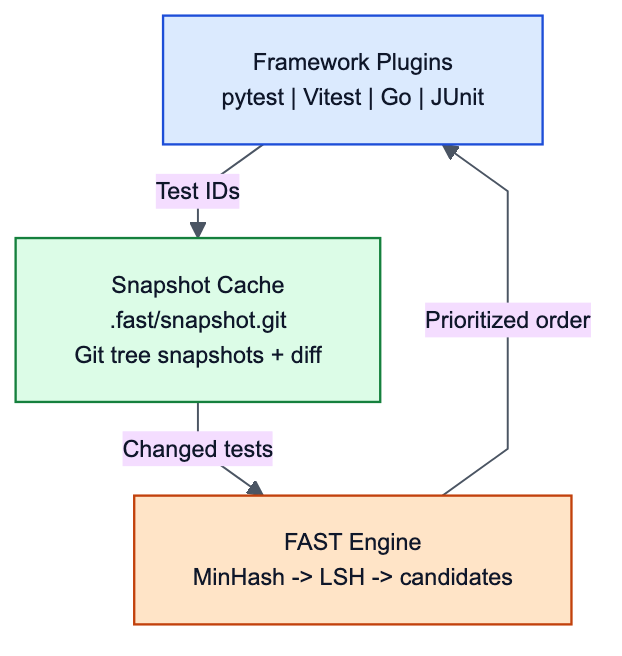
\includegraphics[width=0.34\textwidth]{figures/architecture.png}
\caption{High-level architecture of fast-tcp showing the three main components: framework-specific plugins, the Git-based snapshot cache, and the core FAST engine.}
\label{fig:architecture}
\end{figure}

\textbf{Framework Plugins} provide native integration with testing frameworks. Each plugin intercepts test collection, extracts black-box representations (test identifiers or source content), and reorders test execution based on the prioritized order.

\textbf{Snapshot Cache} maintains a standalone Git repository under \texttt{.fast/snapshot.git} that tracks project state between runs. When prioritization begins, the tool computes a diff against the previous snapshot to identify added, modified, and deleted files.

\textbf{FAST Engine} implements the prioritization algorithms from~\cite{miranda2018fast}, including FAST-pw (pairwise comparison), FAST-one, FAST-log, FAST-sqrt, and FAST-all variants. Each variant trades off precision for speed by selecting different numbers of candidates per iteration.

\subsection{Unique Features}

\subsubsection{Git-based Snapshot Cache}
Unlike traditional approaches that rely on the project's own version control history, fast-tcp maintains an independent snapshot repository. This design choice offers several advantages:

\begin{itemize}
    \item Works in projects without Git or with uncommitted changes
    \item Ignores irrelevant files (build artifacts, caches) automatically
    \item Computes efficient tree diffs using Git's internal algorithms
    \item Prunes old objects to prevent unbounded growth
\end{itemize}

The snapshot cache stores file hashes as Git tree objects, enabling O(n) diff computation where n is the number of tracked files.

\subsubsection{Incremental Prioritization}
When changes are detected, fast-tcp partitions the test suite into three sets: \textit{new} (added or modified), \textit{unchanged} (same content hash), and \textit{deleted} (removed since last run). The prioritization algorithm then:

\begin{enumerate}
    \item Prioritizes new tests first using FAST
    \item Seeds the cumulative signature with new test signatures
    \item Prioritizes unchanged tests using the seeded signature
    \item Returns the combined ordering
\end{enumerate}

This approach ensures that new or modified tests---which are more likely to reveal regressions---execute before unchanged tests.

\begin{figure}[htbp]
\centering
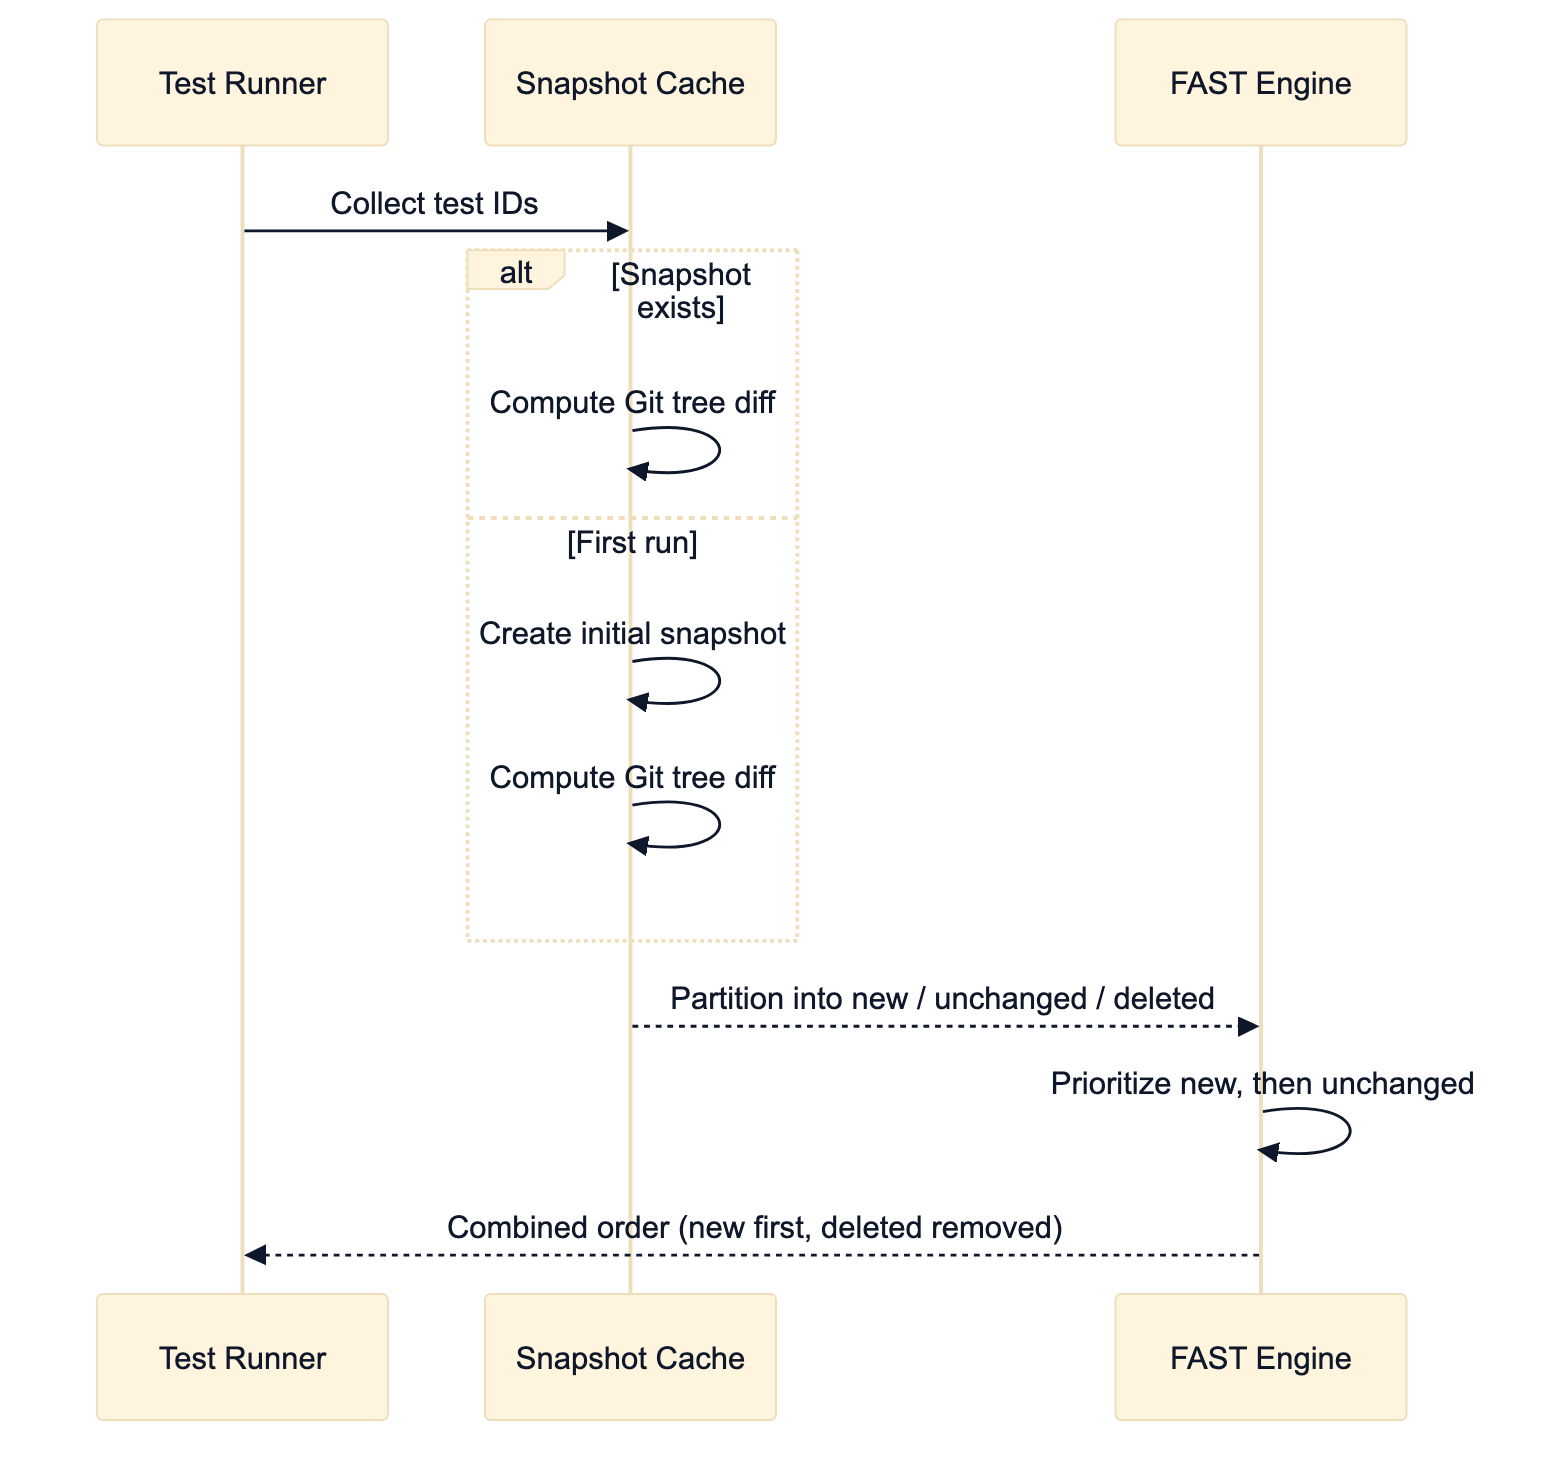
\includegraphics[width=0.40\textwidth]{figures/workflow.png}
\caption{Incremental prioritization workflow. The snapshot cache detects file changes, partitions tests into new/unchanged/deleted sets, and prioritizes new tests first.}
\label{fig:workflow}
\end{figure}

\subsubsection{Multi-Framework Support}
Table~\ref{tab:frameworks} summarizes the supported testing frameworks and their integration mechanisms.

\begin{table}[htbp]
\caption{Supported Testing Frameworks}
\label{tab:frameworks}
\centering
\begin{tabular}{@{}lll@{}}
\toprule
\textbf{Framework} & \textbf{Language} & \textbf{Integration} \\
\midrule
pytest & Python & Plugin (auto-discovered) \\
Vitest & JavaScript/TS & Script helper \\
Go test & Go & Script helper \\
JUnit/Ant & Java & Ant macro \\
\bottomrule
\end{tabular}
\end{table}

\subsection{Implementation and Technology}

fast-tcp is implemented in Python and packaged for PyPI/TestPyPI distribution. Key dependencies include:

\begin{itemize}
    \item \textbf{datasketch}: MinHash and LSH implementations
    \item \textbf{xxhash}: Fast non-cryptographic hashing
    \item \textbf{Git}: Snapshot storage and diff computation
\end{itemize}

Today the repository can be installed directly from source via \texttt{python -m pip install -e .}, and the release workflow is configured for TestPyPI/PyPI publication. The tool targets Python 3.8+.

\subsection{Operational Model}

\subsubsection{pytest Integration}
The pytest plugin provides the simplest integration path. After installation:

\begin{lstlisting}[language=bash,numbers=none]
# Initialize (optional, creates config)
fast-tcp init pytest

# Run with prioritization
pytest --fast-tcp
\end{lstlisting}

The plugin hooks into pytest's collection phase, extracts test node IDs as black-box representations, computes priorities, and reorders the collected items before execution.

\subsubsection{CLI Mode}
For other frameworks or custom workflows, the CLI provides direct access:

\begin{lstlisting}[language=bash,numbers=none]
fast-tcp --test-dir ./tests \
    --algo FAST-pw \
    --entity bbox \
    --repetitions 1
\end{lstlisting}

\section{Demonstration Plan}

During the demonstration, we will showcase fast-tcp through the following scenario:

\begin{enumerate}
    \item \textbf{Setup} (30s): Install fast-tcp from source (or from PyPI once published) and initialize a pytest project with \texttt{fast-tcp init pytest}.
    
    \item \textbf{Baseline Run} (60s): Execute pytest with \texttt{--fast-tcp --fast-tcp-debug} on a sample project containing 50+ tests. Show the debug output with partition, preparation, and prioritization timings.
    
    \item \textbf{Incremental Update} (60s): Modify a single test file and re-run. Demonstrate how the snapshot cache detects the change and prioritizes the modified test first.
    
    \item \textbf{Add New Tests} (60s): Add new test files and show how they receive priority over existing unchanged tests.
    
    \item \textbf{Algorithm Comparison} (60s): Compare FAST-pw (highest search effort) vs FAST-one (smallest candidate sample) on a larger test suite, showing the effectiveness-efficiency tradeoff.
    
    \item \textbf{Multi-Framework} (60s): Briefly demonstrate Vitest integration to show cross-language support.
\end{enumerate}

Key observations attendees will see:
\begin{itemize}
    \item Sub-second prioritization for typical test suites
    \item Automatic change detection without manual configuration
    \item Modified tests appearing first in execution order
    \item Overhead breakdown showing preparation vs prioritization time
\end{itemize}

\begin{figure}[htbp]
\centering
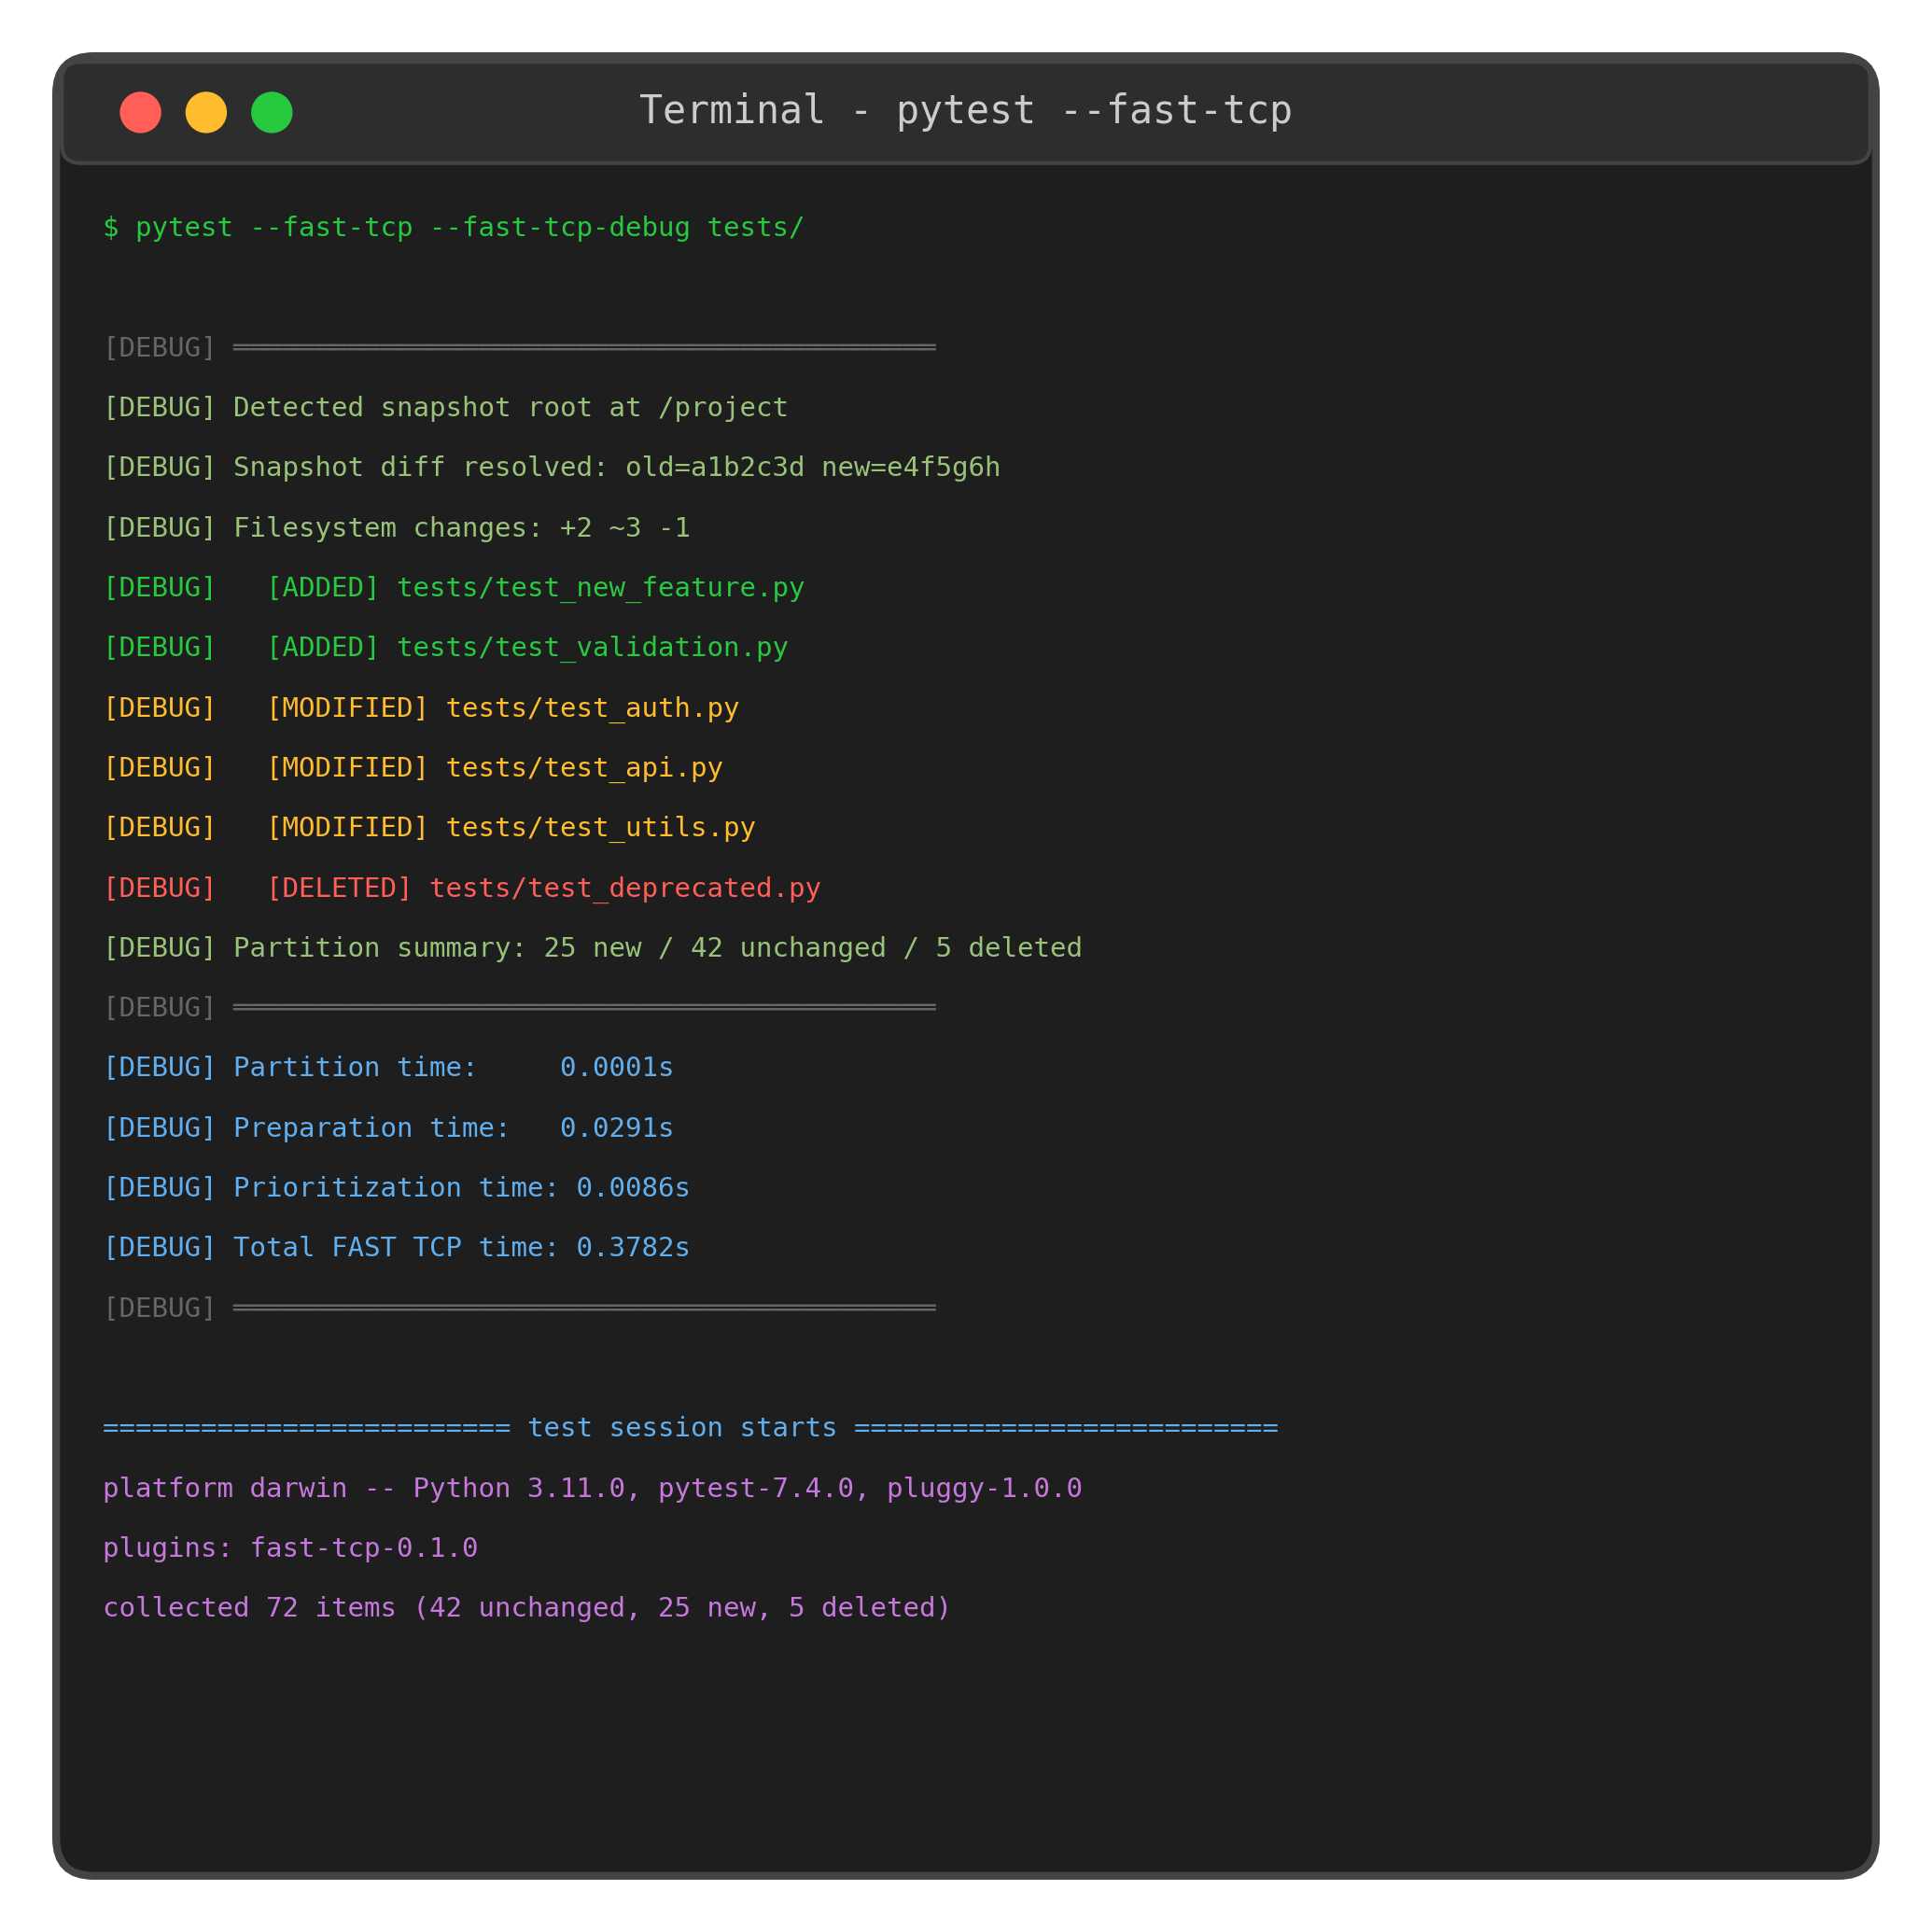
\includegraphics[width=0.48\textwidth]{figures/debug_output.png}
\caption{Sample debug output from pytest with \texttt{--fast-tcp-debug}, showing snapshot diff, test partitioning, and timing breakdown.}
\label{fig:debug}
\end{figure}

\section{Evaluation}

\subsection{Overhead Benchmarks}

To complement the real-project case studies, the artifact bundle includes a profiling-grounded synthetic pytest workload that grows over 20 iterations through additions, modifications, and deletions. Table~\ref{tab:overhead} summarizes that illustrative trace.

\begin{table}[htbp]
\caption{Tool Overhead Benchmark Results}
\label{tab:overhead}
\centering
\begin{tabular}{@{}lr@{}}
\toprule
\textbf{Metric} & \textbf{Value} \\
\midrule
Test suite size (final) & 140 tests \\
Average total overhead & 1.51s \\
Average partition time & 0.1ms \\
Average preparation time & 29ms \\
Average prioritization time & 9ms \\
Overhead range & 1.28s -- 1.77s \\
\bottomrule
\end{tabular}
\end{table}

In this synthetic trace, the majority of end-to-end overhead comes from snapshot and preparation work rather than the FAST ranking step itself. Preparation (signature generation) averages 29ms, while prioritization averages 9ms. This remains consistent with the original FAST observation that prioritization time is dominated by preparation~\cite{miranda2018fast}.

\begin{figure}[htbp]
\centering
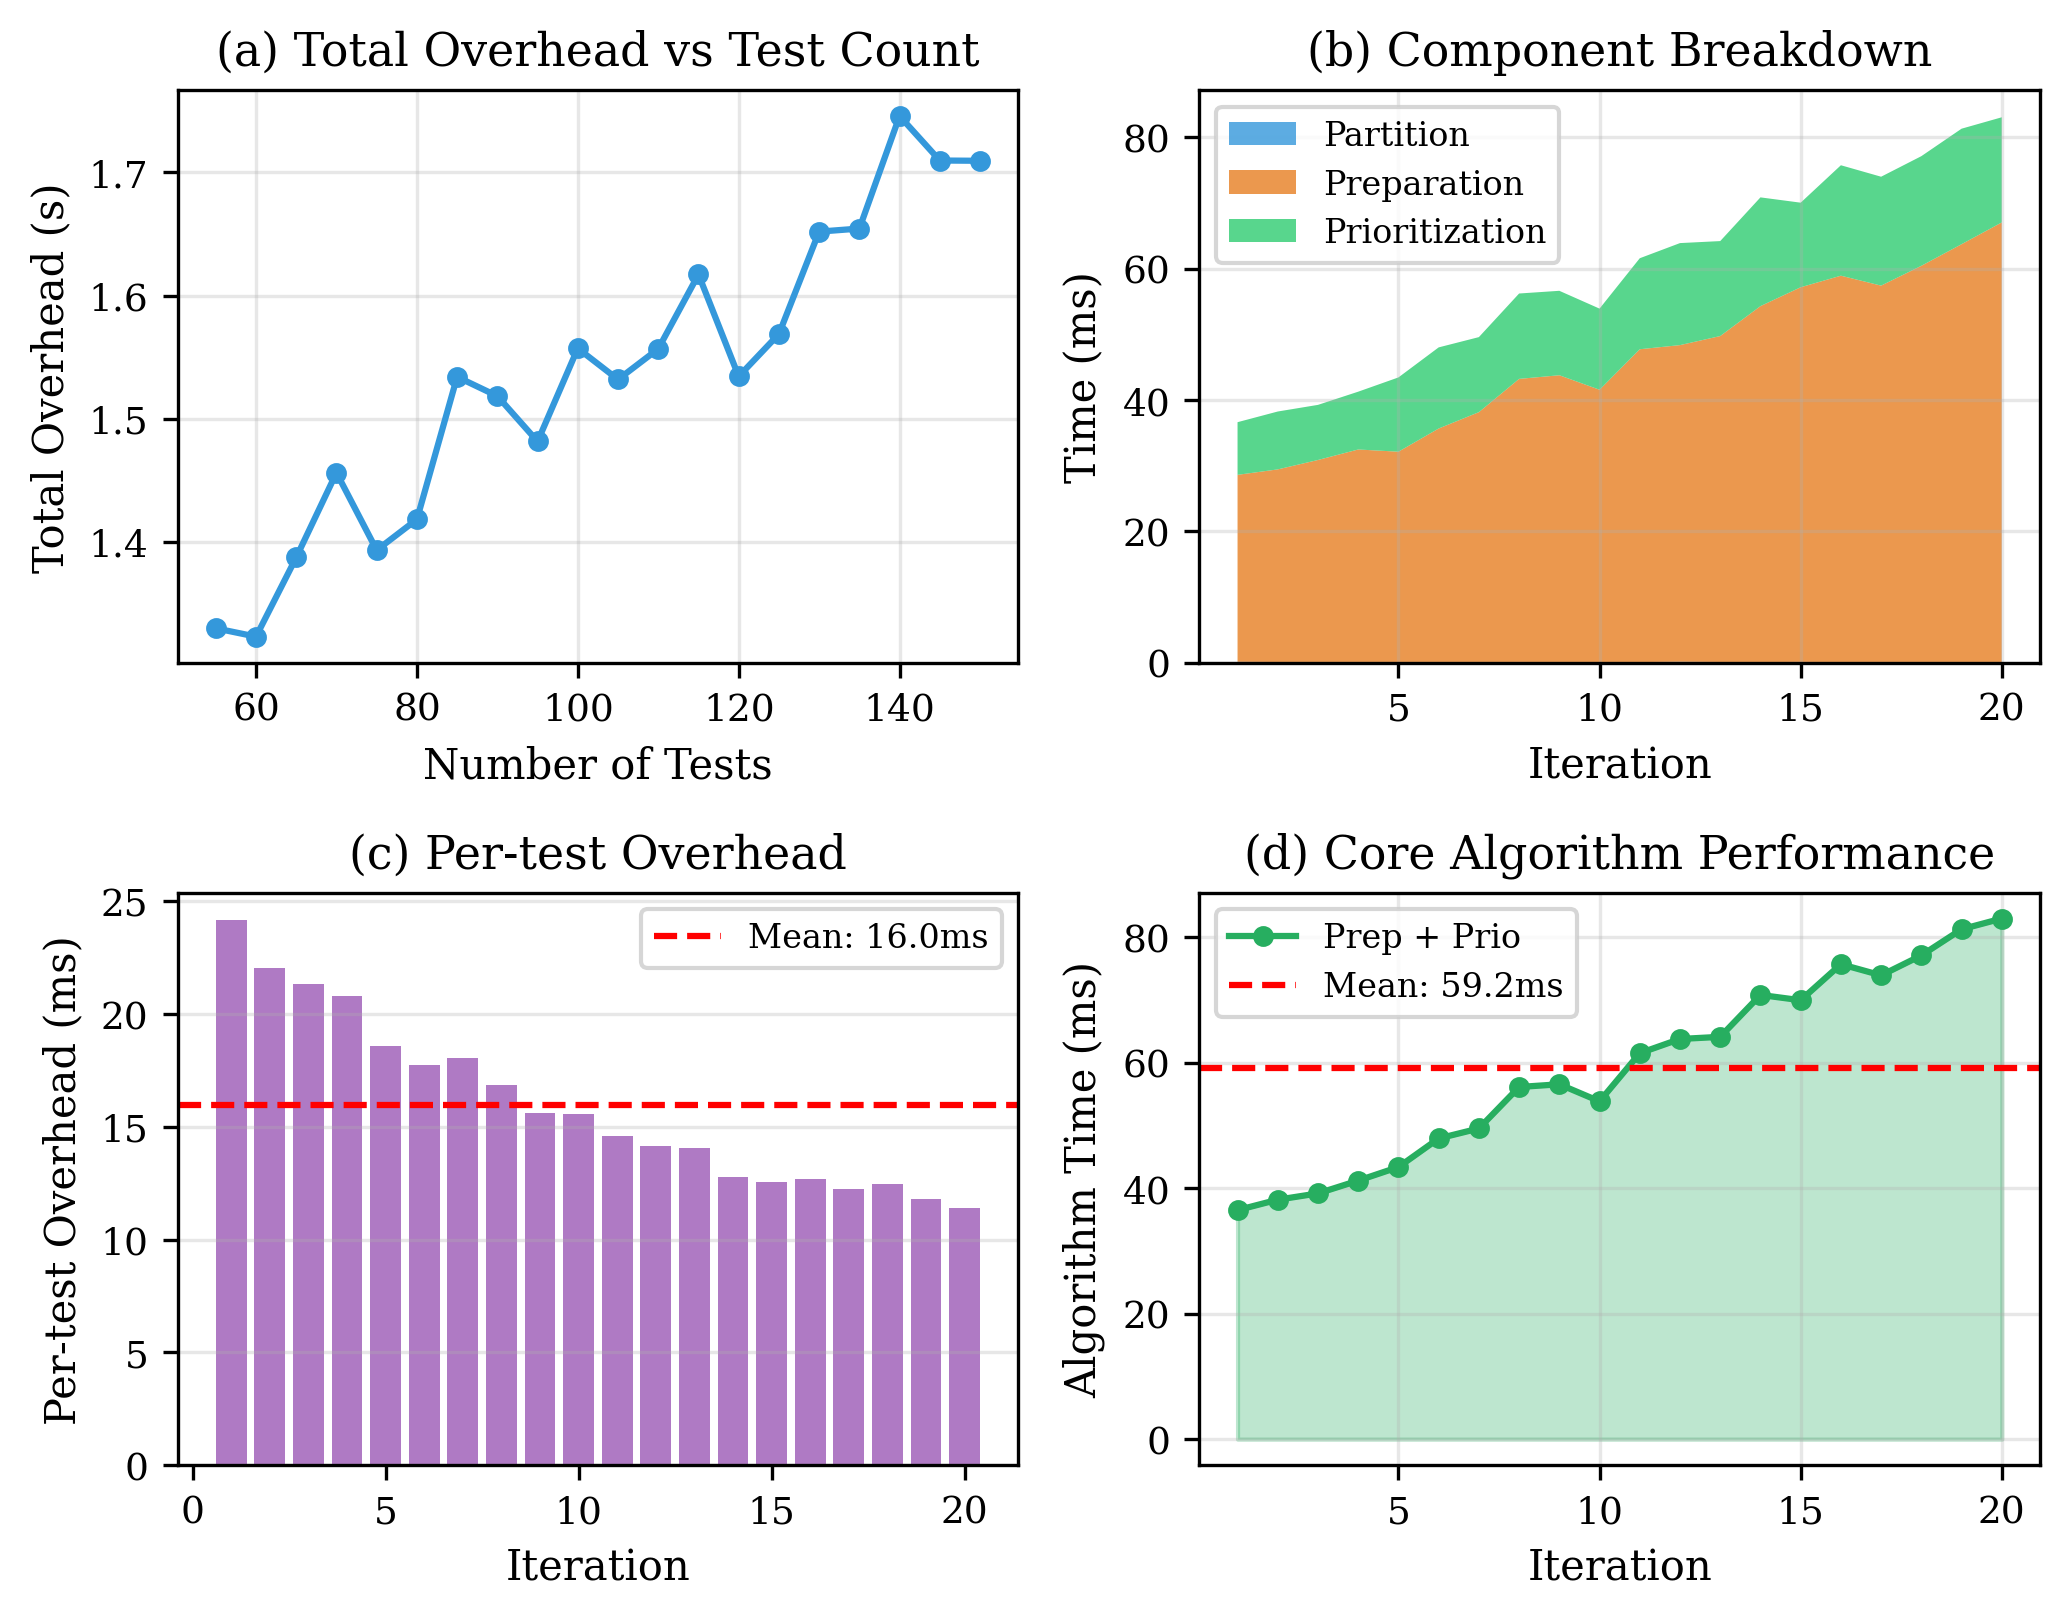
\includegraphics[width=0.48\textwidth]{figures/benchmark_grid.pdf}
\caption{Profiling-grounded synthetic overhead trace over 20 iterations of test suite mutations. (a) Total overhead grows with test count. (b) Time breakdown shows preparation dominates the core FAST step. (c) Per-test overhead remains stable. (d) Core algorithm completes in milliseconds.}
\label{fig:benchmark}
\end{figure}

\subsection{Snapshot Cache Growth}

The artifact bundle also includes a synthetic 40-iteration cache-growth stress scenario (100~MB workspace, 18--32 modifications per iteration). In that scenario, periodic Git garbage collection keeps the repository bounded at roughly 0.26~MB, or about 0.3\% of the working set size.

\subsection{Real-World Case Studies}

To validate practical applicability, we evaluated fast-tcp on four popular open-source Python projects: \texttt{requests} (576 tests), \texttt{rich} (781 tests), \texttt{click} (611 tests), and \texttt{attrs} (1326 tests). Each project was run 5 times with and without fast-tcp enabled. Table~\ref{tab:casestudy} summarizes the results.

\begin{table}[htbp]
\caption{Real-World Case Study Results}
\label{tab:casestudy}
\centering
\begin{tabular}{@{}lrrrr@{}}
\toprule
\textbf{Project} & \textbf{Tests} & \textbf{Baseline} & \textbf{Overhead} & \textbf{\%} \\
\midrule
requests & 576 & 0.57s & 0.60s & 105\% \\
rich & 781 & 4.20s & 0.24s & 6\% \\
click & 611 & 0.90s & 0.46s & 51\% \\
attrs & 1326 & 4.75s & 0.68s & 14\% \\
\bottomrule
\end{tabular}
\end{table}

The absolute overhead ranges from 0.24s to 0.68s across all projects. For projects with longer-running tests (rich, attrs), the relative overhead is low (6--14\%). For projects with very fast test suites (requests, click), the relative overhead is higher but the absolute overhead remains under one second.

\begin{figure}[htbp]
\centering
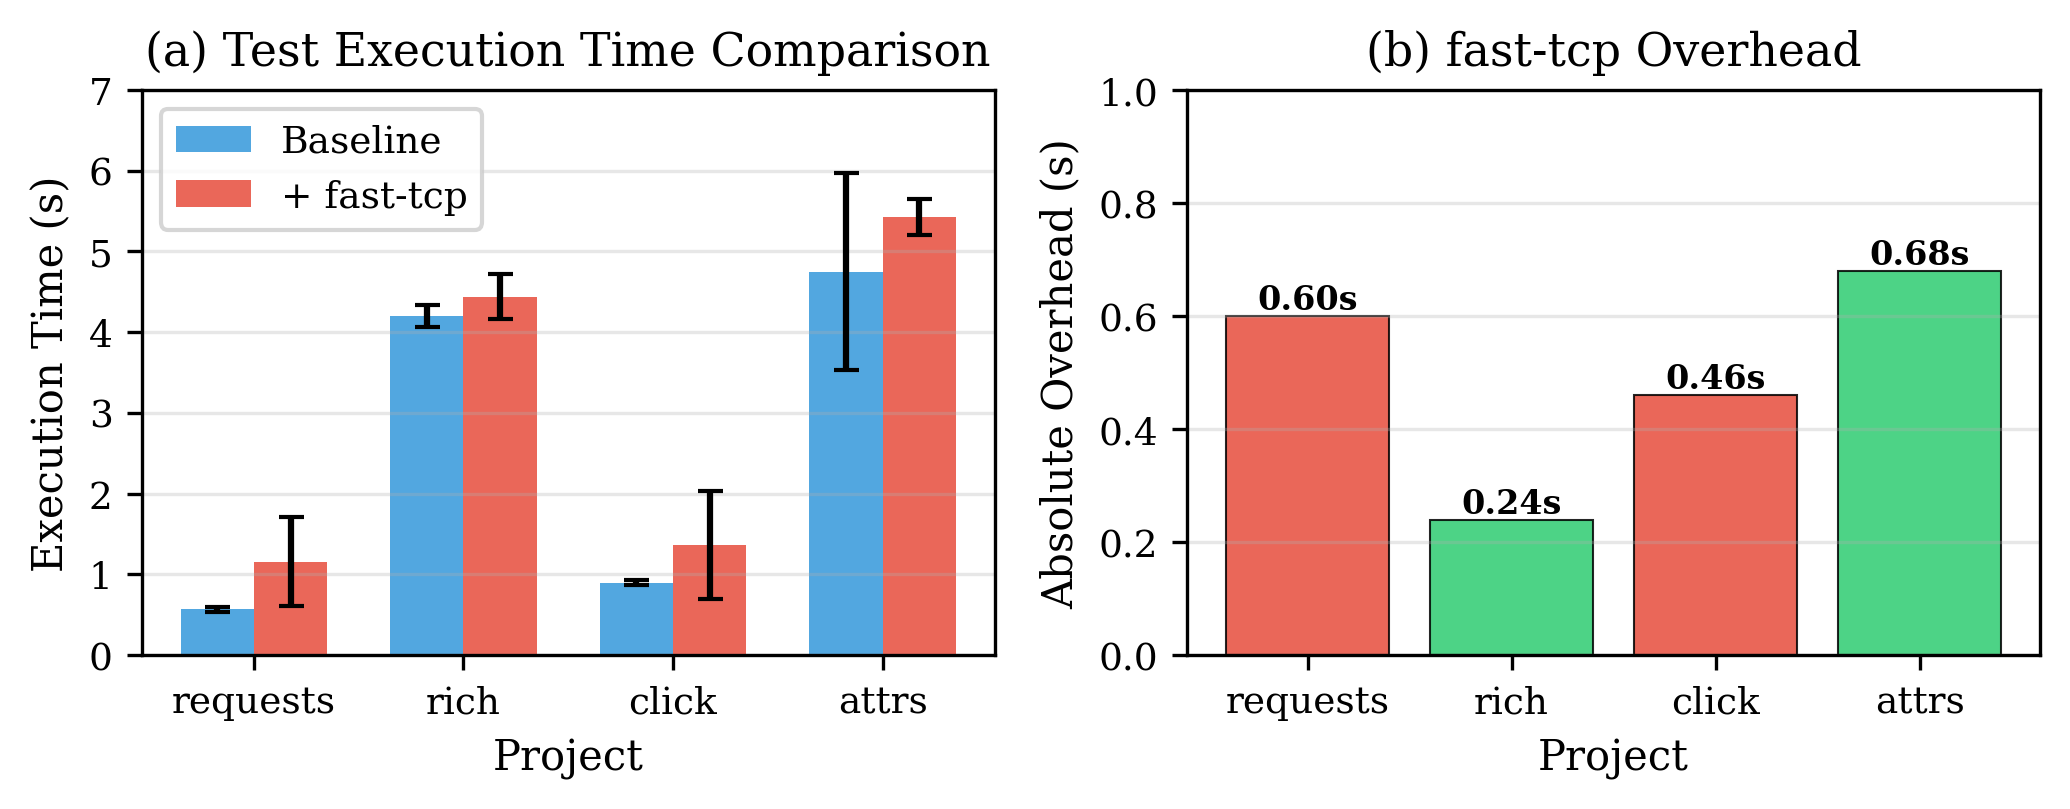
\includegraphics[width=0.48\textwidth]{figures/case_study_bar.pdf}
\caption{Real-world case study results. (a) Execution time comparison between baseline and fast-tcp. (b) Absolute overhead in seconds per project.}
\label{fig:casestudy}
\end{figure}

\subsection{Effectiveness}

fast-tcp preserves the effectiveness characteristics of the original FAST algorithms since it uses identical prioritization logic. Users can select algorithm variants based on their precision-speed tradeoffs:

\begin{itemize}
    \item \textbf{FAST-pw}: Highest search effort, selecting the most dissimilar candidate each iteration
    \item \textbf{FAST-sqrt}: Balanced candidate budget, selecting $\sqrt{n}$ candidates
    \item \textbf{FAST-one}: Lowest search effort, selecting a single candidate per iteration
\end{itemize}

\section{Related Work}

Several tools have addressed test prioritization in practice. Busjaeger and Xie~\cite{busjaeger2016learning} applied machine learning for TCP at Microsoft, using features including coverage and failure history. Elbaum et al.~\cite{elbaum2014techniques} developed strategies for TCP in continuous integration at Google. Both approaches require historical data not always available in practice.

Commercial tools like Buildpulse\footnote{\url{https://buildpulse.io}} provide ML-based test selection and prioritization as cloud services, but require sharing test results with external servers.

fast-tcp differentiates by:
\begin{itemize}
    \item Running entirely locally without external dependencies
    \item Requiring no historical failure data
    \item Supporting incremental prioritization via snapshot caching
    \item Providing a unified tool for multiple testing frameworks
\end{itemize}

\section{Availability and Usage}

fast-tcp is publicly available as source, with release automation prepared for TestPyPI/PyPI publication:

\begin{itemize}
    \item \textbf{Repository}: \url{https://github.com/icse18-FAST/FAST}
    \item \textbf{Package docs}: included in the repository and release metadata
    \item \textbf{Release workflow}: GitHub Actions workflow for TestPyPI/PyPI publication
    \item \textbf{License}: GPL-3.0
\end{itemize}

\noindent\textbf{Quickstart for pytest users:}
\begin{lstlisting}[language=bash,numbers=none]
python -m pip install -e .
cd your-project
fast-tcp init pytest
pytest --fast-tcp
\end{lstlisting}

\noindent\textbf{Requirements:}
\begin{itemize}
    \item Python 3.8 or later
    \item Git (for snapshot caching)
    \item Testing framework of choice
\end{itemize}

\section{Conclusion and Future Work}

We presented fast-tcp, a practical tool that brings similarity-based test case prioritization to developers through maintained framework integrations and intelligent change detection. The tool addresses key adoption barriers by providing lightweight setup, incremental prioritization via Git-based snapshots, and multi-framework support.

Our measured case studies show sub-second absolute overhead across four real projects, while the accompanying synthetic artifact scenarios illustrate the expected cost composition and bounded cache growth. The snapshot cache mechanism enables efficient change detection without relying on the project's own version-control history.

Future work includes:
\begin{itemize}
    \item Support for additional frameworks (Jest, RSpec, NUnit)
    \item Integration with CI/CD platforms (GitHub Actions, GitLab CI)
    \item White-box prioritization using coverage data
    \item Distributed prioritization for very large test suites
\end{itemize}

\balance

\bibliographystyle{IEEEtran}
\begin{thebibliography}{10}

\bibitem{miranda2018fast}
B.~Miranda, E.~Cruciani, R.~Verdecchia, and A.~Bertolino, ``{FAST} approaches to scalable similarity-based test case prioritization,'' in \emph{Proc. ICSE'18: 40th International Conference on Software Engineering}, 2018, pp. 222--232.

\bibitem{elbaum2014techniques}
S.~Elbaum, G.~Rothermel, and J.~Penix, ``Techniques for improving regression testing in continuous integration development environments,'' in \emph{Proc. FSE'14}, 2014, pp. 235--245.

\bibitem{memon2017taming}
A.~Memon, Z.~Gao, B.~Nguyen, S.~Dhanda, E.~Nickell, R.~Siemborski, and J.~Micco, ``Taming Google-scale continuous testing,'' in \emph{Proc. ICSE-SEIP'17}, 2017, pp. 233--242.

\bibitem{busjaeger2016learning}
B.~Busjaeger and T.~Xie, ``Learning for test prioritization: An industrial case study,'' in \emph{Proc. FSE'16}, 2016, pp. 975--980.

\end{thebibliography}

\end{document}
